\subsection{Frontend}
Per eliminare un meeting, è necessario aprire il relativo \texttt{Dialog} per visualizzarne i dettagli. 
A questo punto, è presente il pulsante \textit{elimina}. 
L'immagine seguente mostra il pulsante quando vi si passa sopra con il mouse.
\begin{figure}[H]
    \centering
    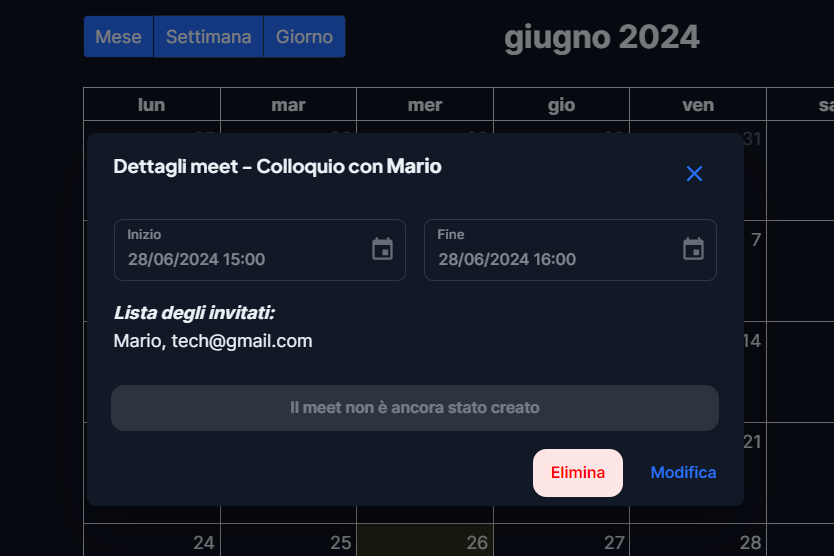
\includegraphics[width=\textwidth]{EliminaMeet/hoverEliminaMeet.png}
    \caption{Eliminazion meet - hover}
\end{figure}
\noindent Se si clicca sul pulsante, viene visualizzato un popup di conferma:
\begin{figure}[H]
    \centering
    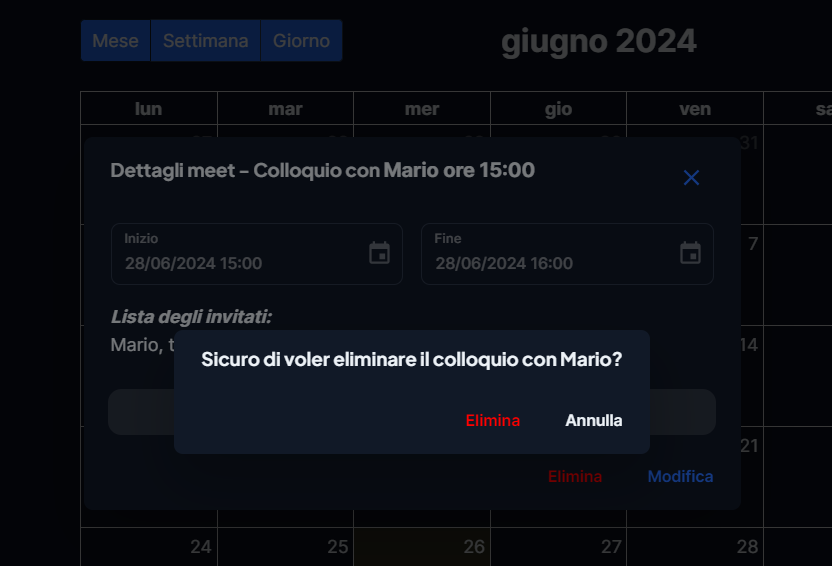
\includegraphics[width=\textwidth]{EliminaMeet/popupConfermaEliminazione.png}
    \caption{Eliminazion meet - popup di conferma}
\end{figure}
\noindent Proseguendo con l'eliminazione, viene chiamata la funzione \texttt{handleDelete}
\begin{lstlisting}[language=typescript, frame=lines, basicstyle=\ttfamily\scriptsize, numbers=left]
const handleDelete = async () => {
    setOpen(false);
    setOpenDeleteMeetDialog(false);
  
    const payload = {
        id: eventDetails.id,
        webexId: eventDetails.extendedProps.webexId,
    };
  
    try {
        const response = await deleteMeeting(payload);
  
        if (response.status == 200) {
          const updatedEvents = events.filter((event) => event.id != eventDetails.id);
          setEvents(updatedEvents);
  
          showPopup('Eliminazione avvenuta con successo', true);
        } else {
          showPopup("Errore nell'eliminazione del meeting", false);
        }
    } catch (error) {
        console.error("Errore durante l'eliminazione di un evento:", error);
        showPopup("Errore nell'eliminazione del meeting", false);
    }
};
\end{lstlisting}
\begin{itemize}
    \item \textbf{Righe 6-7}:  viene creato il payload da inviare al backend, 
    contenente i due ID necessari per l'eliminazione del meeting: l'ID del database e l'ID di Webex.

    \item \textbf{Righe 14-15}: se l'eliminazione è andata a buon fine, l'array degli eventi associati a \texttt{Fullcalendar} 
    viene aggiornato manualmente. Questo avviene creando un nuovo array tramite la funzione \texttt{filter}, 
    che rimuove l'evento con lo stesso ID di quello eliminato. In questo modo, il cambiamento viene immediatamente visualizzato
    nel calendario senza bisogno di ricaricare la pagina.
\end{itemize}
Se il meet viene eliminato con successo, viene mostrato un popup di avviso:
\begin{figure}[H]
    \centering
    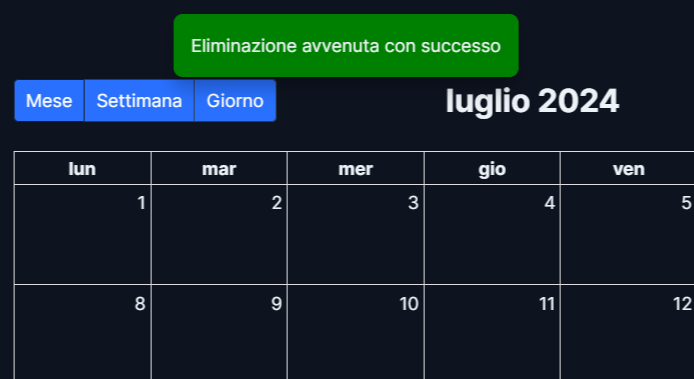
\includegraphics[width=\textwidth]{EliminaMeet/popupSuccessoEliminazione.png}
    \caption{Eliminazion meet - popup di successo}
\end{figure}
